%********************************************************************
% Appendix
%*******************************************************
% If problems with the headers: get headings in appendix etc. right
%\markboth{\spacedlowsmallcaps{Appendix}}{\spacedlowsmallcaps{Appendix}}
\chapter{Appendix C: Supplementary Information of Chapter 5}

\begin{refsection}[referencesCh4]
\section{Environmental geographic information model} \label{section:Section1AppC}
\subsection{Trophic State Index} \label{section:TSIAppC}
\citet{carlson_trophic_1977} proposed the Trophic State Index (TSI) as a metric to determine the trophic status of waterbodies. This is used by the U.S. Environmental Protection Agency (US EPA) \citep{QAPP2012}. This index can be calculated using three parameters: concentration of chlorophyll-$\alpha$ (chl-$\alpha$), concentration of total phosphorus, and water turbidity measured through the Secchi depth. Only the two first methods has been used in this work since they are less affected to exogenous phenomena (such as atmospheric conditions, or variations in the flow of water streams). Correlations to compute the TSI from these parameters are shown in Eq. \ref{eq:TSI_clh_AppC} and \ref{eq:TSI_TP_AppC}, where $Clh$ denotes the concentration of chlorophyll-$\alpha$, and $TP$ denotes the concentration of total phosphorus in $\sfrac{mg}{m^3}$ \citep{carlson_trophic_1977}. 

The TSI of a waterbody is scored in a range from zero to one hundred, which can be correlated with the oligotrophic, mesotrophic, eutrophic and hypereutrophic classes as shown in Table \ref{table:ApCTSI_relation_AppC}. Oligotrophic and mesotrophic denote low and intermediate biomass productivities, while eutrophic and hypereutrophic are referred to waterbodies with high biological productivity and frequent algal blooms. Combined data for chl-$\alpha$ and total phosphorus concentrations retrieved from the National Lakes Assessments (NLA) carried out by the US EPA in the years 2007 and 2012 \citep{NLA2012, NLA2007} is used to determine the Trophic State Index of lentic waters in the contiguous U.S, as shown in Fig. \ref{fig:ApCTSImap_AppC}. No TSI values are assigned to the watersheds without reported data.

\begin{align}
& \text{TSI}_{\text{chl-$\alpha$}} = 10  \cdot \left(6-\frac{2.04-0.68 \cdot \text{ln}\left(Clh\right)}{\left(2\right)}\right) \label{eq:TSI_clh_AppC} \\
& \text{TSI}_{\text{TP}} = 10  \cdot \left(6-\frac{\text{ln}\left(\frac{48}{TP}\right)}{\left(2\right)}\right) \label{eq:TSI_TP_AppC}
\end{align}

\begin{table}[h]
	\centering
	\caption{Relation between TSI value and trophic class.}
	\label{table:ApCTSI_relation_AppC}
	\resizebox{0.8\columnwidth}{!}{
	\begin{tabular}{@{}lllll@{}}
		\toprule
		{TSI}           & \textless 40 & 40-50       & 50-70     & \textgreater{}70 \\ \midrule
		{Trophic Class} & Oligotrophic & Mesotrophic & Eutrophic & Hypereutrophic   \\ \bottomrule
	\end{tabular}}
\end{table}

\begin{figure}[h]
	\centering
	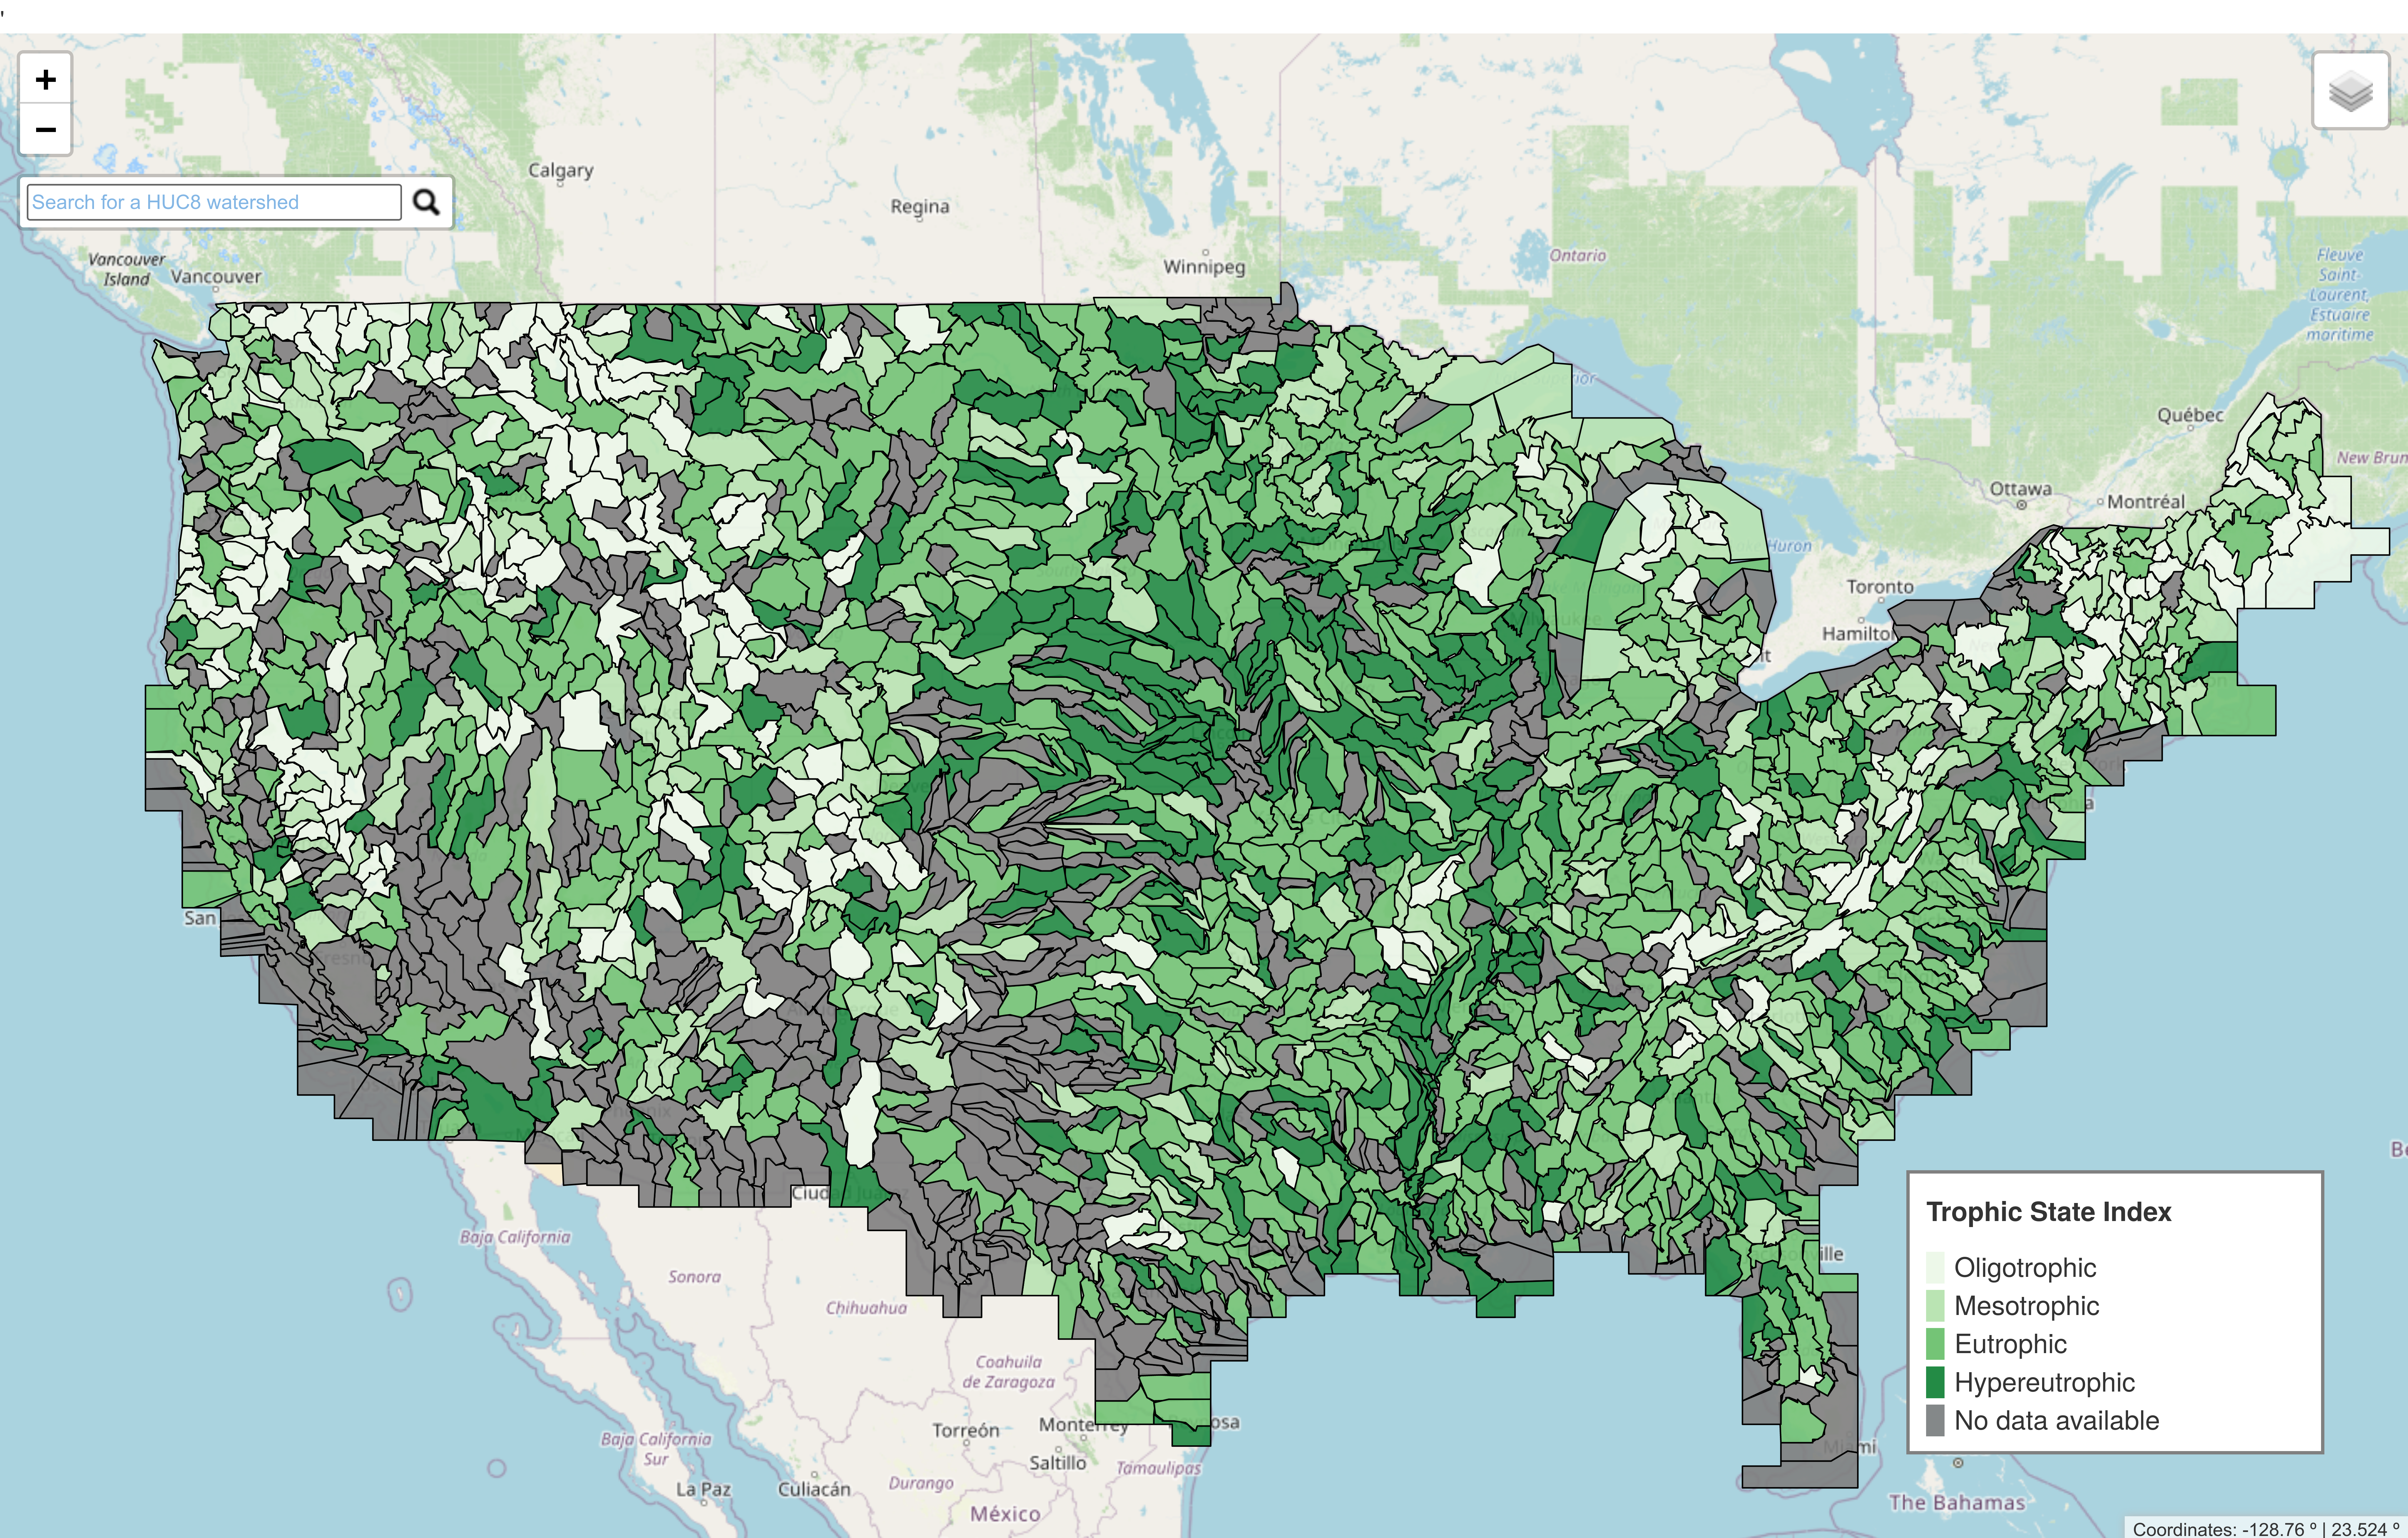
\includegraphics[width=0.95\textwidth, trim={0cm 0cm 0cm 0cm},clip]{gfx/AppendixC/TrophicStateIndex.pdf} 
	\caption{Trophic State Index in the contiguous US HUC8 watersheds.}
	\label{fig:ApCTSImap_AppC}
\end{figure}

\subsection{Balance of anthropogenic phosphorus releases}
Agricultural releases are a main source of human-based phosphorus releases due to the excessive use of synthetic fertilizers and livestock waste for nutrient supplementation in croplands \citep{Dzombak}. Since this work is limited to the assessment of agricultural phosphorus releases, other possible sources of phosphorus releases are not considered. Agricultural phosphorus releases have been estimated from data reported by the Nutrient Use Geographic Information System (NuGIS) project. Further information about the methodology used for the estimation of human-based phosphorus releases can be found in \citet{NuGIS}.

The anthropogenic phosphorus uptakes considered are those due to the crops grown in each watershed. In addition, phosphorus retained by wetlands is considered. Data from \citet{USDAHandbook} is used to estimate the phosphorus uptakes of different crops, attending to their different phosphorus requirements and yield rates. To determine the crops grown in each watershed, the land cover uses are first determined using data from the US EPA EnviroAtlas database for the most recent year available (2011), differentiating between croplands, pasturelands, wetlands, and developed areas (urban areas) \citep{EnviroAtlas}. To estimate the distribution of crops in croplands, including corn, soybeans, small grains, cotton, rice, vegetables, orchards, greenhouse and other crops (i.e., fruits, sugar crops, and oil crops) \citep{2017CensusofAgriculture}, data from the 2017 U.S. Census of Agriculture is used. In case of two or more crops were harvested from the same land during the year (double cropping), the area was counted for each crop. Since the data from the 2017 U.S. Census of Agriculture are published at HUC6 resolution, they have been reconciled to HUC8 level by the fraction of occupied area by each HUC8 watershed in the corresponding HUC6 watershed. The wetlands phosphorus uptake value assessed is 0.77 gP m$^{-2}$ year$^{-1}$, based on data reported by \citet{Kadlec}.

\begin{figure}[h]
	\centering
	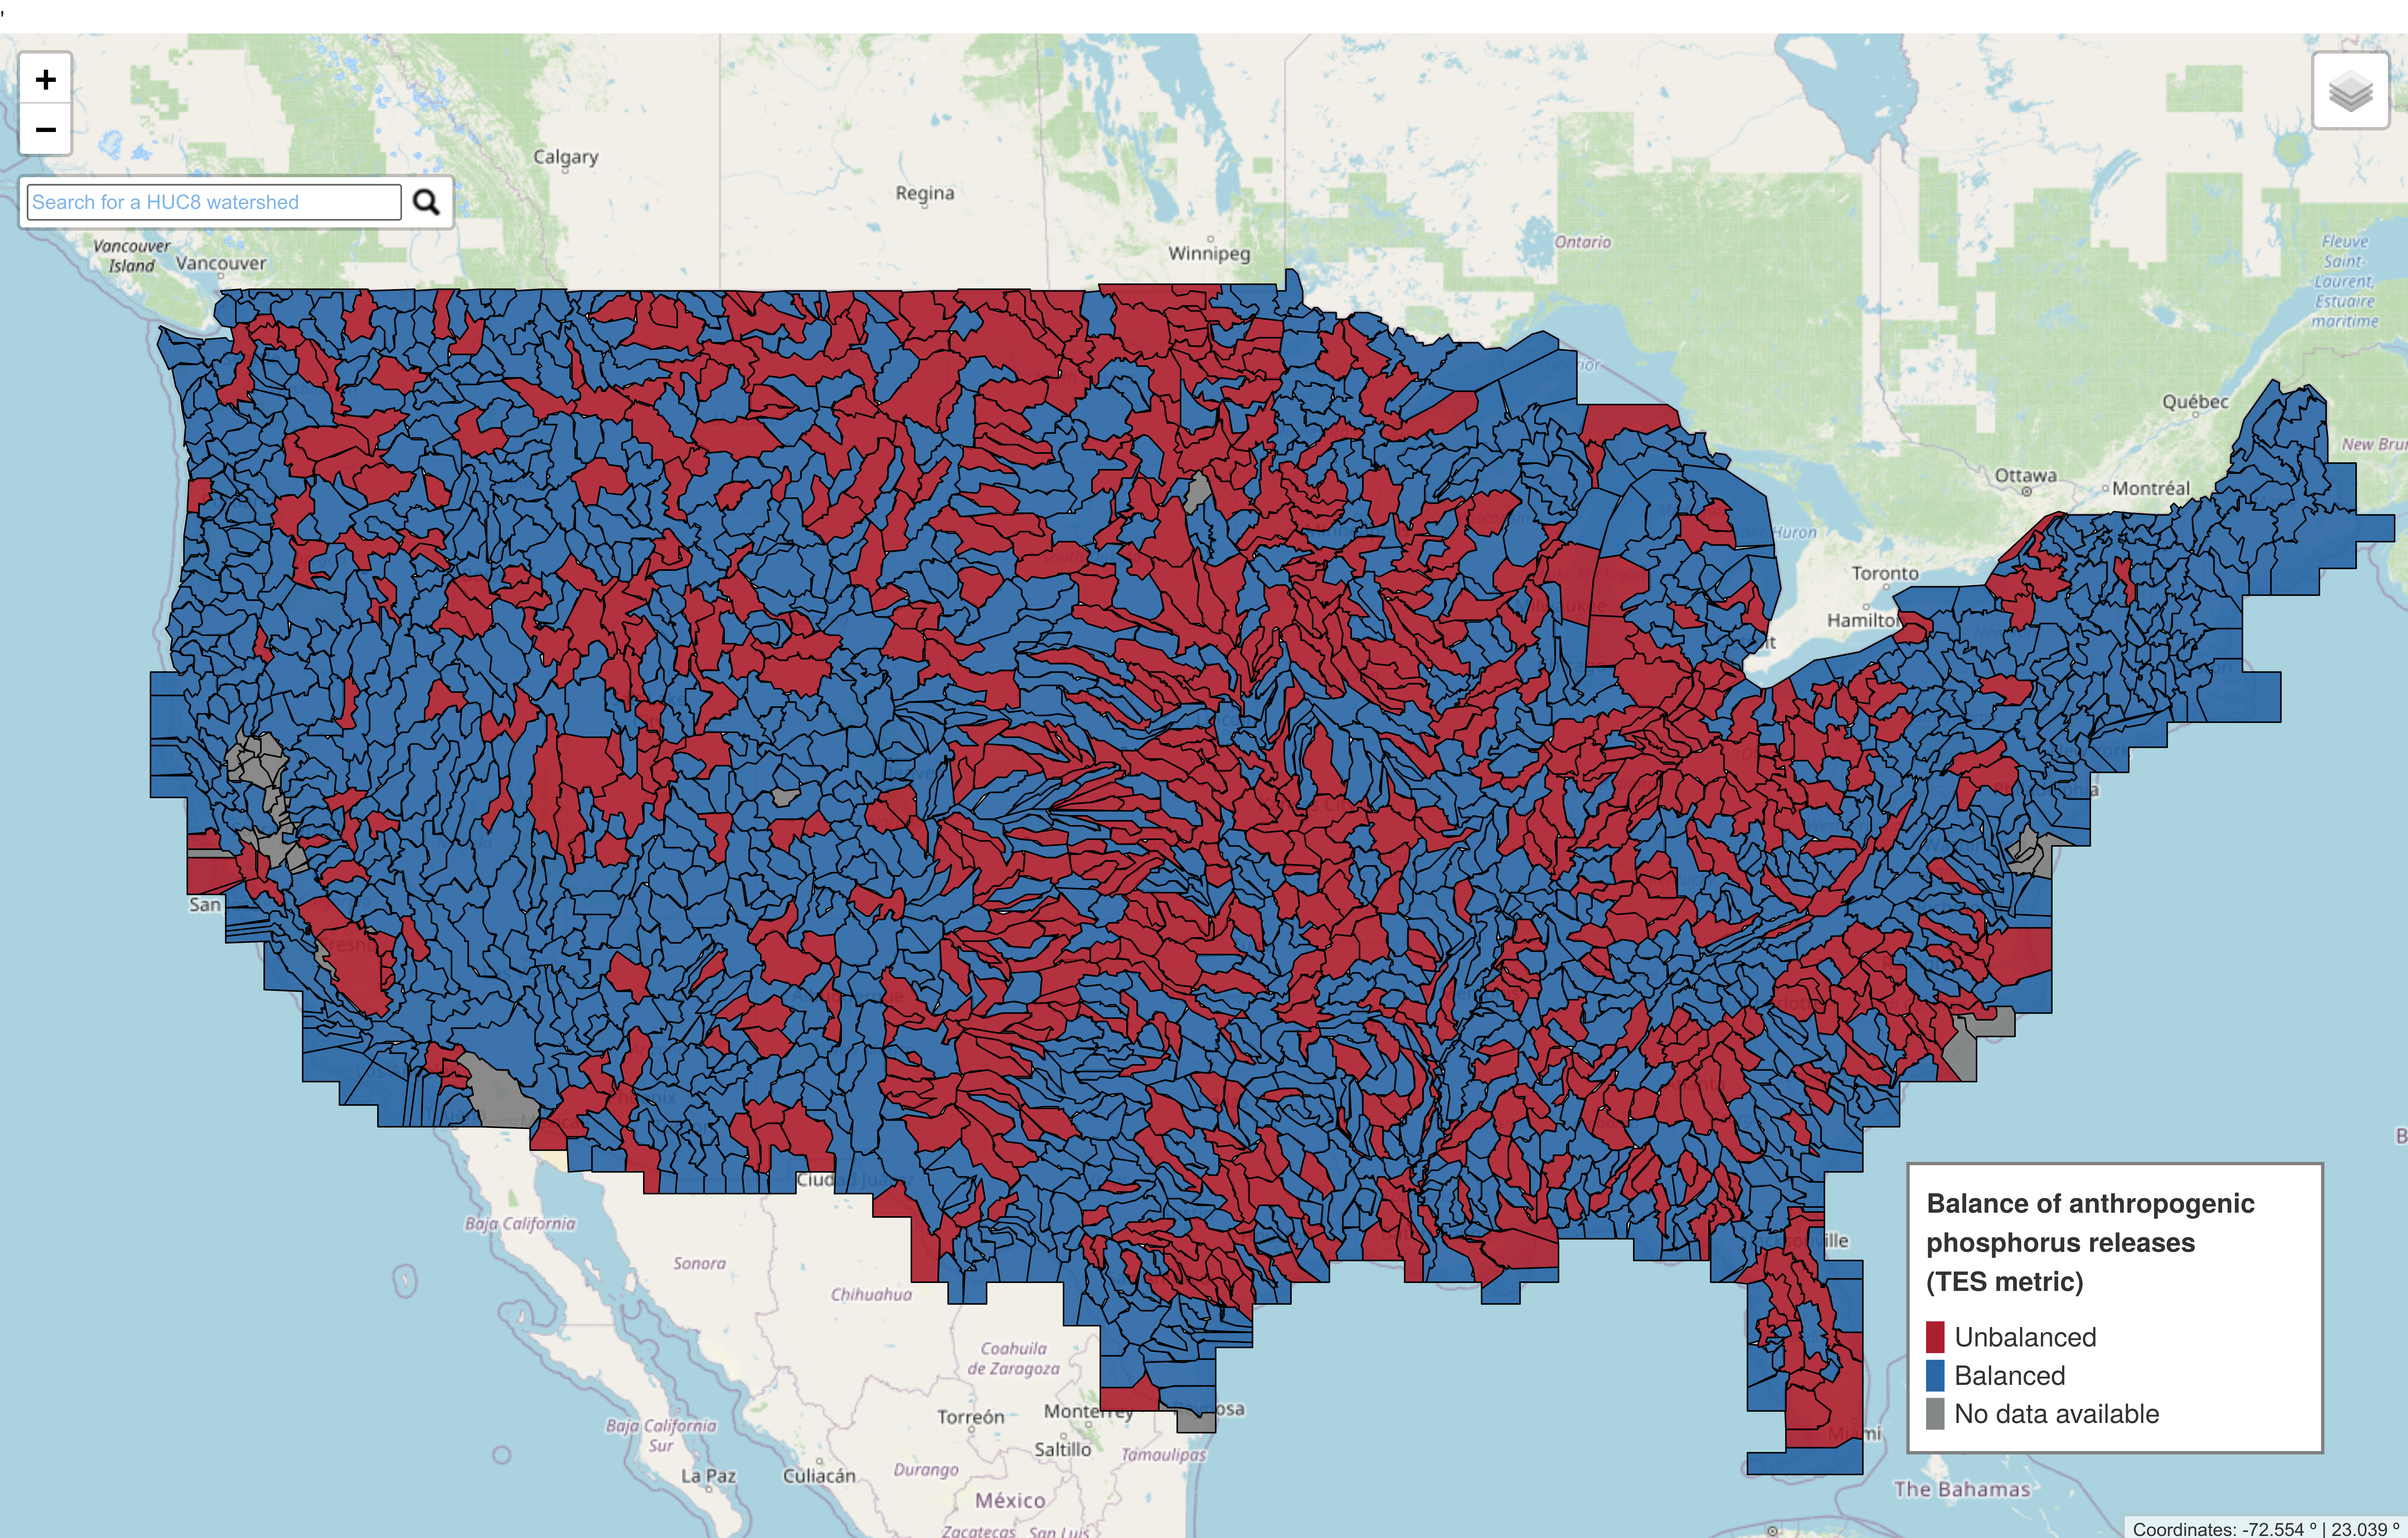
\includegraphics[width=0.95\linewidth, trim={0cm 0cm 0cm 0cm},clip]{gfx/AppendixC/BalanceofP.pdf} 
	\caption{Balance of anthropogenic phosphorus releases in the contiguous US at a HUC8 spatial resolution.}
	\label{fig:TECmap_AppC}
\end{figure}

\subsection{Phosphorus in soils}
Phosphorus concentration in soils is considered to evaluate the legacy phosphorous continuously builds-up in soils. However, only a fraction of phosphorus is available for plants. To measure this phosphorus fraction available for plants, several standardized phosphorus soil tests have been proposed, including Olsen, Bray 1 and Mehlich 3 tests. Among them,  Mehlich 3 (M3P) has been selected as a measure of the concentration of P in soils since it is a widely used metric, and it is the P soil test least affected by changes in soil pH. To estimate the fraction of phosphorus available for plants from total phosphorus concentration data, a correlation developed by \citet{AllenMallarino2006} has been used, Eq. \ref{eq:ApCMehlich3_AppC}. However, this correlation has been developed for agricultural soils in Iowa. Due to the lack of wider studies in this regard, the M3P estimations calculated for the contiguous U.S. must be considered as an exploratory effort to determine the phosphorus saturation in soils across the the contiguous U.S. in an attempt to select the most suitable nutrients management technology according to the geographic environmental indicators. Datasets for samples from the soil A horizon published by the U.S. Geological Survey (USGS) in the ``Geochemical and Mineralogical Data for Soils of the Conterminous United States'' report were used to evaluate the concentration of total phosphorus along the contiguous U.S. \citep{SoilsUSGS}.
\begin{align}
& \text{M3P} \ (\% \text{ over TP}) = \frac{4.698 \cdot 10^{-1}}{1+\left(\text{TotalP} \ (\text{mg}/\text{kg}) \cdot 1.336 \cdot 10^{-3}\right)^{-2.148}} \label{eq:ApCMehlich3_AppC}
\end{align}

The relationship between M3P test value and the quality of soil is shown in Table \ref{table:ApCsoil_fertility_AppC}. Soil fertility levels below optimum indicate that nutrient supplementation is needed to enhance the yield of crops, optimum values indicates that no nutrient supplementation is needed, and excessive soil fertility level indicate over-saturation of phosphorus in soil that can reach waterbodies by runoff \citep{Espinoza2006}.

\begin{table}[h]
	\centering
	\caption{Relation between Mehlich 3 phosphorus and soil fertility level \protect\citep{Espinoza2006}.}
	\label{table:ApCsoil_fertility_AppC}
	\resizebox{0.9\columnwidth}{!}{
	\begin{tabular}{@{}cc@{}}
		\toprule
		Soil Fertility Level & M3P soil phosphorus concentration (ppm) \\ \midrule
		Very Low             & \textless{}16                           \\
		Low                  & 16-25                                   \\
		Medium               & 26-35                                   \\
		Optimum              & 36-50                                   \\
		Excessive            & \textgreater{}50                        \\ \bottomrule
	\end{tabular}}
\end{table}


\begin{figure}[h]
	\centering
	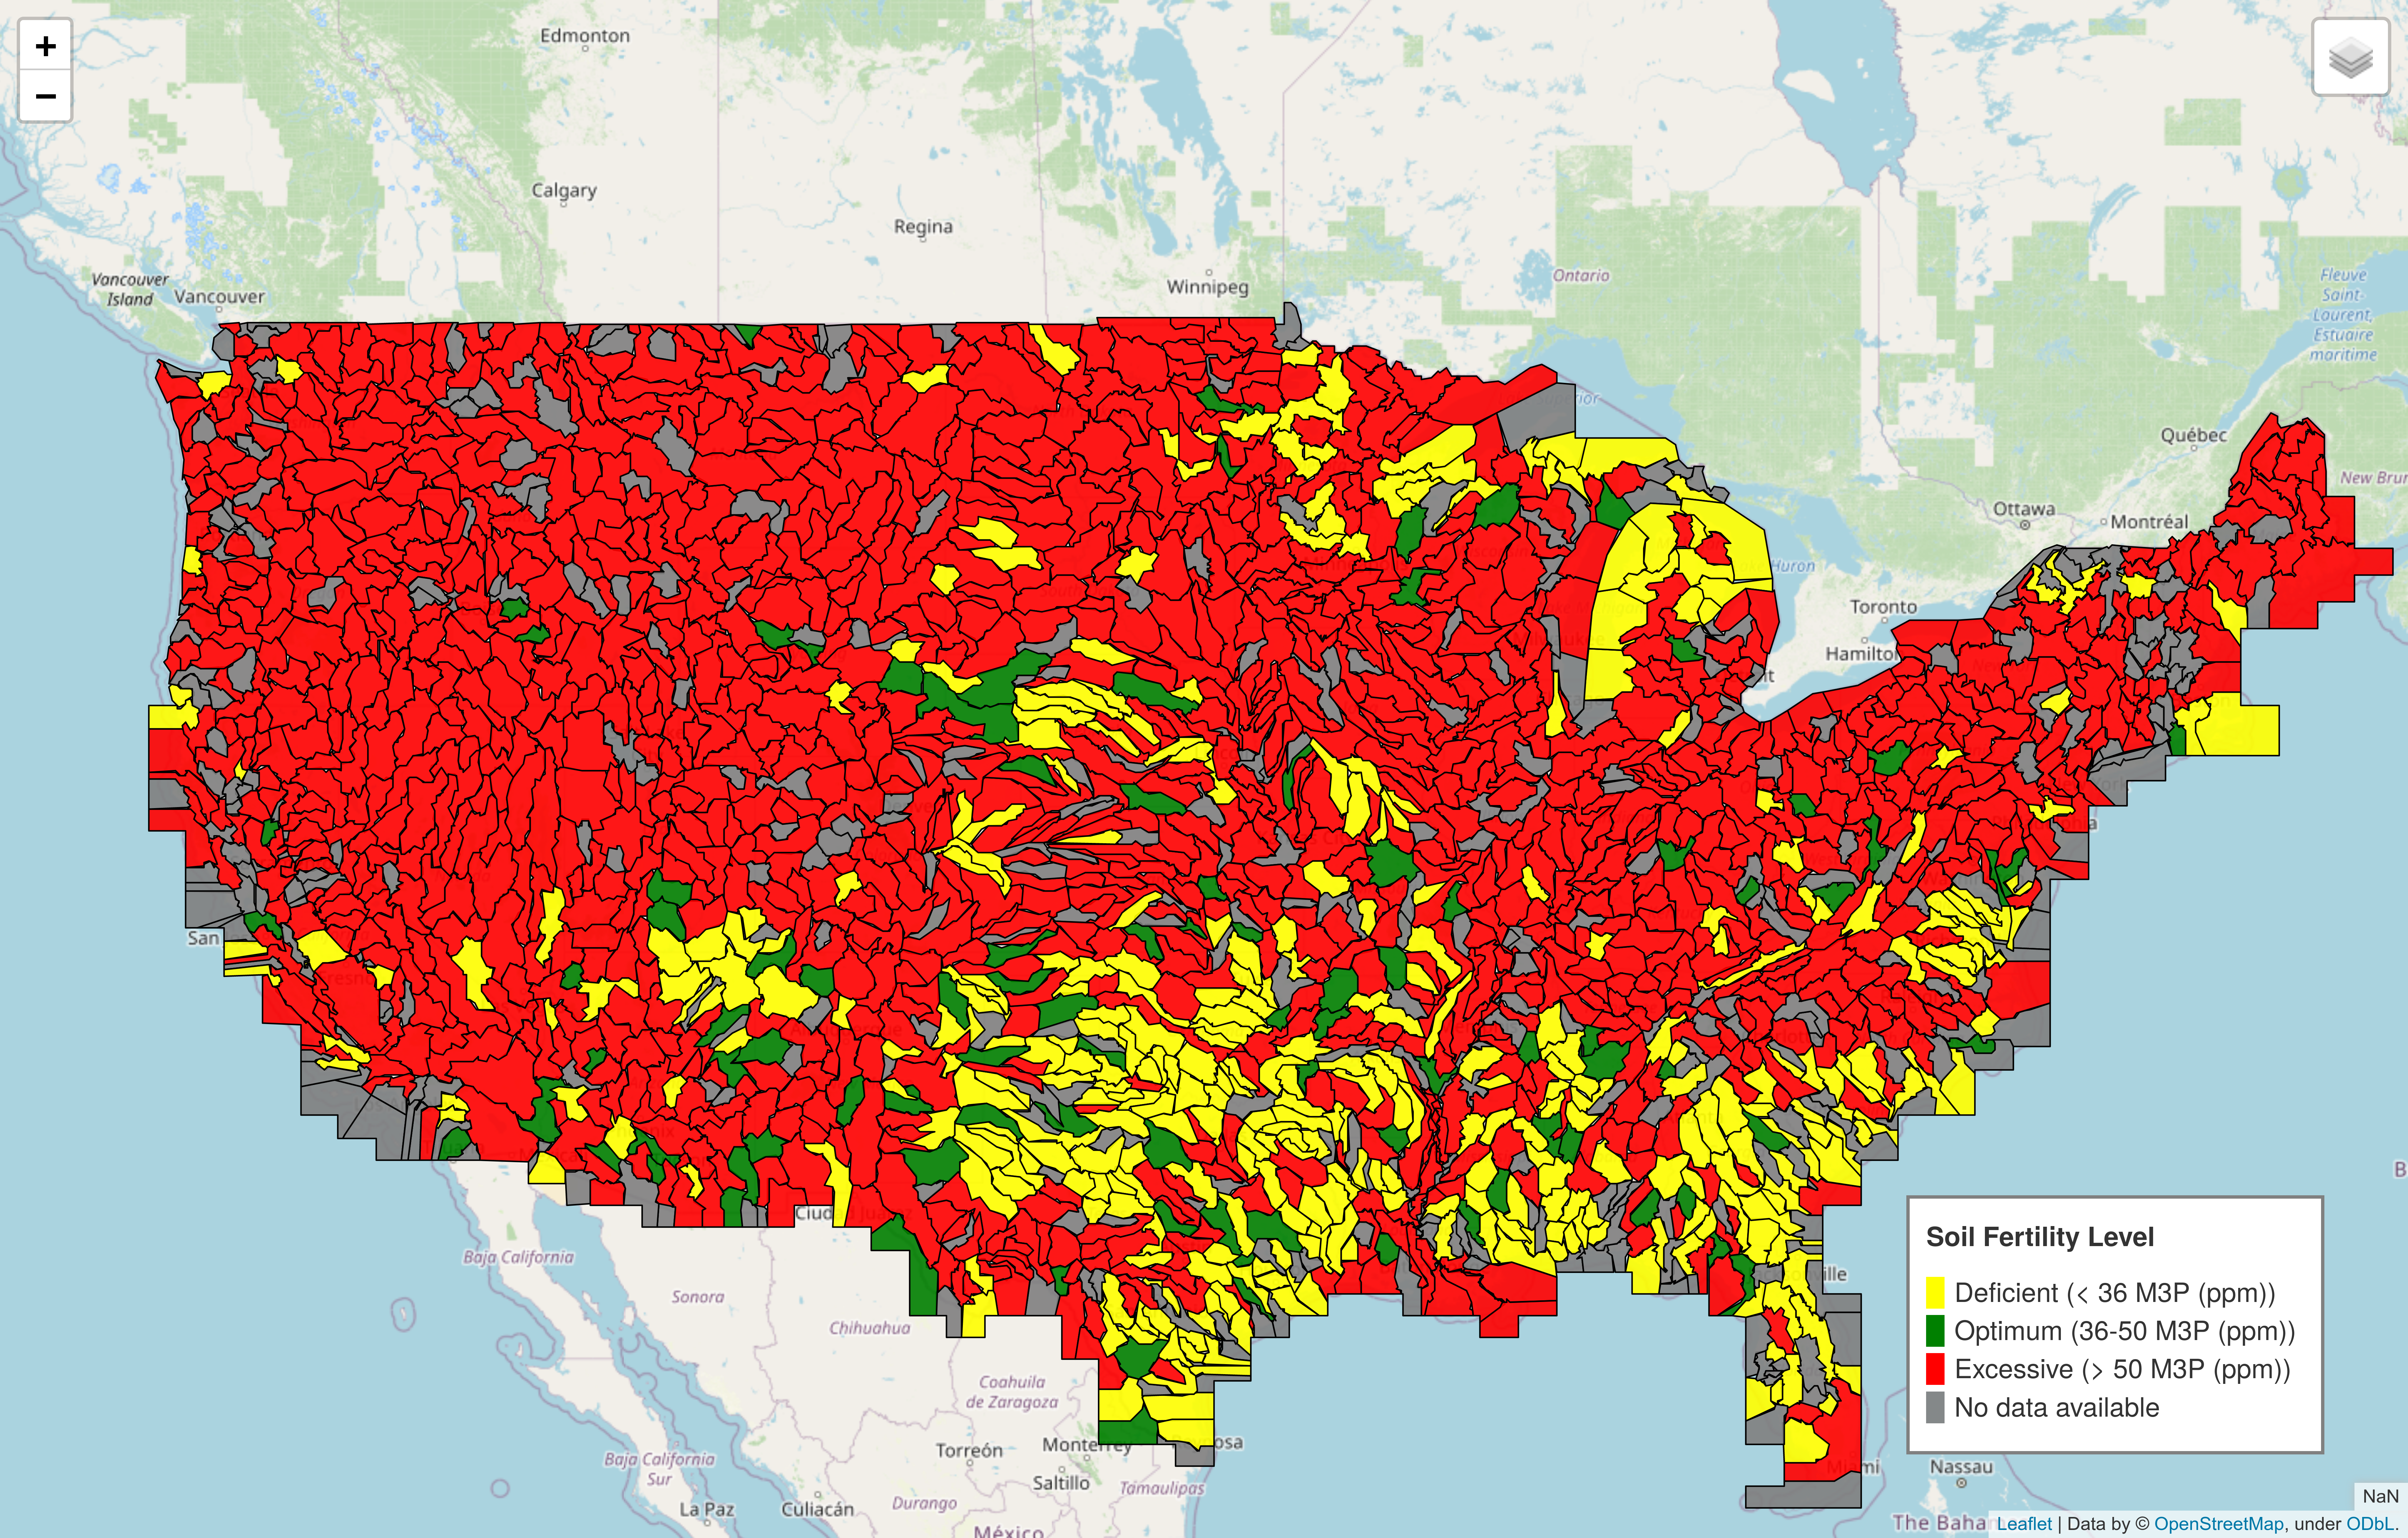
\includegraphics[width=0.95\linewidth, trim={0cm 0cm 0cm 0cm},clip]{gfx/AppendixC/SoilFertility.pdf} 
	\caption{Soil Fertility Level in the contiguous US at a HUC8 spatial resolution.}
	\label{fig:SoilFertilitySoilFertility_AppC}
\end{figure}

\section{Framework development}
\subsection{Data entry}

\begin{table}[h]
	\centering
	\caption{Livestock waste composition and generation rates for different types of animals \protect\citep{Kellog2010, USDAHandbook}.}
	\label{table:manure_characteristics_AppC}
	\resizebox{\columnwidth}{!}{
		\begin{tabular}{@{}ccccccccc@{}}
			\toprule
			\begin{tabular}[c]{@{}c@{}}Livestock\\ type\end{tabular} & \begin{tabular}[c]{@{}c@{}}Water\\ (\%wt)\end{tabular} & \begin{tabular}[c]{@{}c@{}}Organic\\ matter (\%wt)\end{tabular} & \begin{tabular}[c]{@{}c@{}}Total N\\ (\%wt)\end{tabular} & \begin{tabular}[c]{@{}c@{}}Total P\\ (\%wt)\end{tabular} & \begin{tabular}[c]{@{}c@{}}Total Ca\\ (\%wt)\end{tabular} & \begin{tabular}[c]{@{}c@{}}Total K\\ (\%wt)\end{tabular} & \begin{tabular}[c]{@{}c@{}}Generation\\ rate (kg/day)\end{tabular} & \begin{tabular}[c]{@{}c@{}}Animal unit\\ equivalence\end{tabular} \\ \midrule
			Dairy cow                                                & 87                                                     & 10,98                                                           & 0,59                                                     & 0,08                                                     & 0,12                                                      & 0,20                                                     & 37,88                                                              & 0,74                                                              \\
			Dairy heifer                                             & 83                                                     & 13,04                                                           & 0,48                                                     & 0,09                                                     & 0,12                                                      & 0,21                                                     & 29,95                                                              & 0,94                                                              \\
			Dairy calf                                               & 83                                                     & 9,28                                                            & 0,51                                                     & 0,06                                                     & 0,12                                                      & 0,13                                                     & 29,95                                                              & 4,00                                                              \\
			Beef cow                                                 & 88                                                     & 10,58                                                           & 0,34                                                     & 0,08                                                     & 0,12                                                      & 0,24                                                     & 28,58                                                              & 1,00                                                              \\
			Beef calf                                                & 88                                                     & 10,00                                                           & 0,58                                                     & 0,10                                                     & 0,12                                                      & 0,38                                                     & 28,14                                                              & 4,00                                                              \\ \bottomrule
	\end{tabular}}
\end{table}

\begin{table}[h]
	\centering
	\caption{Predefined economic parameters.}
	\label{table:economic_parameters_AppC}
	\resizebox{0.5\columnwidth}{!}{
	\begin{tabular}{@{}cc@{}}
		\toprule
		Parameter                                                                                                & Value \\ \midrule
		\begin{tabular}[c]{@{}c@{}}Discount rate\\ (\%)\end{tabular}                                             & 7     \\
		\begin{tabular}[c]{@{}c@{}}Phosphorus credits\\ (USD / kg P recovered)\end{tabular}                      & 22    \\
		\begin{tabular}[c]{@{}c@{}}Electricity price\\ (Renewable Energy Certificates) \\ (USD/MWh)\end{tabular}  & 60    \\
		\begin{tabular}[c]{@{}c@{}}Bio-methane price\\ (Renewable Identification Number) \\ (USD/kg)\end{tabular} & 1.25  \\
		\begin{tabular}[c]{@{}c@{}}Capital cost incentive\\ (\% over total capital cost)\end{tabular}            & 0     \\ \bottomrule
	\end{tabular}}
\end{table}

\subsection{Techno-economic model}
\subsubsection{Manure conditioning model}
U.S. EPA determines that the content of total solids in manure should be less than 15\%, as shown in Fig. \ref{fig:TS_max_AppC} \citep{AgSTARHandbook}. Therefore, additional water may be added to reduce the solids content in manure before the anaerobic digestion stage.
\begin{figure}[h]
	\centering
	\includegraphics[width=0.85\linewidth, trim=1cm 4cm 1cm 2.5cm, clip]{gfx/AppendixC/water_manure_properties} 
	\caption{Adequate manure properties for anaerobic digestion. Adapted from \protect\citet{AgSTARHandbook}.}
	\label{fig:TS_max_AppC}
\end{figure}

\subsubsection{Anaerobic digestion model}
\begin{table}[h] 
	\centering
	\caption{Statistical summary of nutrients composition for cattle manure before and after anaerobic digestion (AD). All concentrations are reported in mg/L. TKN is referrered to total Kjeldahl nitrogen, and TP to total phosphorus. Data from \protect\citet{ADAS,Martin2,Alburquerque,Sorensen}.} \label{table:nut_mod_AppC}
	\resizebox{\columnwidth}{!}{
		\begin{tabular}{ccccccccc}
			\toprule
			{} 	  &  \begin{tabular}[c]{@{}c@{}}TKN\\ before AD\end{tabular} & \begin{tabular}[c]{@{}c@{}}TKN\\ after AD\end{tabular} 	&  \begin{tabular}[c]{@{}c@{}}NH\textsubscript{4}\\ before AD\end{tabular} 			&  \begin{tabular}[c]{@{}c@{}}NH\textsubscript{4}\\ after AD\end{tabular}  				&  \begin{tabular}[c]{@{}c@{}}TP\\ before AD\end{tabular}  &			  \begin{tabular}[c]{@{}c@{}}NH\textsubscript{4}\\ after AD\end{tabular}  &  			\begin{tabular}[c]{@{}c@{}}P-PO\textsubscript{4}\\ before AD\end{tabular} &  			\begin{tabular}[c]{@{}c@{}}P-PO\textsubscript{4}\\ after AD\end{tabular}    \\
			\midrule
			count &    10.00 &        10.0 &     10.00 &                10.00 &                5.00 &                5.00 &                 5.00 &                 5.00    \\      
			mean  &   3856.10 &      3967.1 &  1845.90 &              2340.10 &             1442.60 &             1449.60 &               811.40 &               946.40    \\      
			std   &   847.41 &       942.9 &    354.59 &               387.34 &              467.14 &              485.29 &               277.67 &               331.88    \\      
			min   &   2920.00 &     2800.0 &    1300.00 &              1810.00 &              813.00 &              838.00 &               457.00 &               562.00   \\    
			25\%   &  3050.00 &     3152.5 &    1607.50 &              2047.50 &             1170.00 &             1170.00 &               590.00 &               670.00   \\  
			50\%   & 3660.00 &     3855.0 &     1825.00 &              2340.00 &             1450.00 &             1360.00 &               880.00 &               950.00   \\
			75\%   & 4630.75 &      4882.5 &    2159.75 &              2590.00 &             1860.00 &             1920.00 &              1050.00 &              1260.00   \\
			max   &     4960.00 &   5290.0 &     2300.00 &              2881.00 &             1920.00 &             1960.00 &              1080.00 &              1290.00  \\
			\bottomrule
	\end{tabular}}
\end{table}

Correlations to estimate the capital cost, Eq. \ref{eq:inv_costs_AppC}, and operating and management costs (O\&M), Eq. \ref{eq:OM_costs_AppC}, as a function of the animal population of CAFOs were developed using data from the US EPA AgSTAR program \citep{AgSTAR2003} and the USDA \citep{USDA_OM} respectively, as shown in Figure \ref{fig:AD_size_2cost_AppC}. It should be noted that O\&M cost does not include the capital cost amortization. Therefore, to estimate the total production cost, the annualized equipment cost has been added to the O\&M costs, Eq.  \ref{eq:OM_inv_costs_AppC}. The assumed equipment lifetime is 20 years.

\begin{align} 
& \text{Installation cost (MM USD (2019))} = \label{eq:inv_costs_AppC} \\
& \left(4.271 \cdot 10^{-4} \cdot N_{animals}+0.127\right) \cdot 1.511 \nonumber \\ \nonumber\\
%	& \frac{\text{O\&M}} {\text{Installation cost}} \text{ ratio} = \frac{15858.710}{(1+\left(N_{animals} \cdot 13.917\right)^{1.461}} \label{eq:OM_costs}\\ \nonumber\\
& \frac{\text{O\&M}} {\text{Installation cost}} \text{ ratio} = \frac{15.858\cdot 10^{3}}{(1+\left(N_{animals} \cdot 13.917\right)^{1.461}} \label{eq:OM_costs_AppC}\\ \nonumber\\
& \text{Operating cost} = \text{O\&M costs} + \frac{\text{Investment cost}}{\text{Plant lifetime}} \label{eq:OM_inv_costs_AppC}
\end{align}

\begin{figure}[h!]
	\centering
	\begin{subfigure}[t]{0.7\textwidth}
		\includegraphics[width=\textwidth, trim={0cm 0cm 0cm 0cm},clip]{gfx/AppendixC/AD_size_cost}
		\caption{Cost of AD units as a function of the number of animals (cattle). Data from \citet{AgSTAR2003}.}
		\label{fig:AD_size_cost_AppC}
	\end{subfigure}
	\bigskip
	\begin{subfigure}[t]{0.75\textwidth}
		\includegraphics[width=\textwidth]{gfx/AppendixC/AD_size_OM_Unit_cost} 
		\caption{O\&M costs as a function of the number of animals (cattle). Data from \citet{USDA_OM}.}
		\label{fig:AD_size_OM_Unit_cost_AppC}
	\end{subfigure}
	
	\caption{Correlations between AD capital and O\&M costs, and the number of cattle in the livestock facility.}
	\label{fig:AD_size_2cost_AppC}
\end{figure}

\subsubsection{Solid-liquid separation model}
Based on the evaluation reported by \citet{MollerSLsep}, a screw press is the technology selected to carry out the solid-liquid separation stage since it is the most cost efficient liquid-solid equipment. The partition coefficients for the different components are shown in Table \ref{table:part_coef_AppC}.
\begin{table}[h] 
%	\begin{adjustwidth}{}{}
		\centering
		\caption{Partition coefficients for solid-liquid manure separation using a screw press unit \protect\citep{MollerSLsep}.} \label{table:part_coef_AppC}
		\resizebox{0.6\columnwidth}{!}{
		\begin{tabular}{c c c}
			\toprule
			Element 	& Solid fraction & Liquid fraction	\\ \midrule
			Total mass 	& 0.08		& 0.92 \\
			Dry matter 	& 0.31		& 0.69 \\
			Org. N 		& 0.09		& 0.91 \\
			Org. P		& 0.22	 	& 0.78 \\ \bottomrule
		\end{tabular}
%	\end{adjustwidth}
	}
\end{table}

To determine the commercial sizes and number of units necessary as a function of the flow to be treated, data from commercial manufacturers is considered \citep{PWTech}. The feasible configurations in terms of screw press diameter and number of units as a function of the waste flow treated are shown in Table \ref{table:ScrewPress_units_AppC}. Data reported by \citet{Matches} for this type of equipment is used to relate the unit diameter and cost, while the operating costs are calculated assuming power consumption reported by the manufacturer for each model, as shown in Fig. \ref{fig:screwpress_investment_costs_AppC} and Table \ref{table:ScrewPress_power_AppC}.
\begin{table}[h] 
%	\begin{adjustwidth}{}{}
		\centering
		\caption{Sizing estimated for screw press units based on commercial data \protect\citep{PWTech}.} \label{table:ScrewPress_units_AppC}
		\resizebox{\columnwidth}{!}{
		\begin{tabular}{c c c c c}
			\toprule
			\multicolumn{1}{c}{Load capacity $\left(\frac{m^{3}}{day}\right)$}&\multicolumn{4}{c}{Number of units}\\
			\cmidrule(lr){2-5}
			&\diameter(m) 0.23 & \diameter(m) 0.35 & \diameter(m) 0.42 & \diameter(m) 0.56	\\ \midrule
			$<$ 43 		& 1 	& - 					& - & -	\\
			43 - 81 	& -						& 1 	& - & - 	\\
			81 - 190 	& -						& - 					& 1 & - 	\\
			190 - 381 	& -						& -					 	& 2 & -	\\ 
			381 - 572 & -						& -					 	& 3 & - 	\\ 
			572 - 708 & -						& -					 	& - & 2	 	\\ 
			708 - 1090 & -						& -					 	& - & 3	 	\\
			1090 - 1444 & -						& \-				 	& - & 4	 	\\
			$>$ 1444 	&-						& -					 	& - & $\ceil[\bigg]{\frac{\text{Flow } \left(\sfrac{m^{3}}{day}\right)}{\text{Load Capacity}_{\text{\diameter 0.56m unit}}}}$  	\\\bottomrule
		\end{tabular}
%	\end{adjustwidth}
	}
\end{table}

\begin{figure}[h!]
	\centering
	\includegraphics[width=0.75\linewidth, trim={0.5cm 0cm 0cm 0cm},clip]{gfx/AppendixC/screwpress_cost_m} 
	\caption{Estimated screw press investment costs (USD) as a function of the size.}
	\label{fig:screwpress_investment_costs_AppC}
\end{figure}

\begin{table}[h] 
%	\begin{adjustwidth}{}{}
		\centering
		\caption{Electrical power of screw press units \protect\citep{PWTech}.} \label{table:ScrewPress_power_AppC}
		\resizebox{0.7\columnwidth}{!}{
		\begin{tabular}{c c c c c}
			\toprule
			\multicolumn{1}{c}{Number of units } &\multicolumn{4}{c}{Electrical power (kW)}\\
			\cmidrule(lr){2-5}
			&\diameter(m) 0.23 & \diameter(m) 0.35 & \diameter(m) 0.42 & \diameter(m) 0.56	\\ \midrule
			1 		& 0.3 & 0.45 & 0.9 & -	\\
			2 	& -						& - 	& 1.27 & 3.88 	\\
			3	& -						& - 					& 2.01 & 6.34 	\\
			4 	& -						& - 					& - & 7.83 \\
			\bottomrule
		\end{tabular}
%	\end{adjustwidth}
	}
\end{table}

\begin{figure}[h!]
	\centering
	\begin{subfigure}[t]{0.7\linewidth}
		\centering
		\includegraphics[width=\linewidth]{gfx/AppendixC/screwpress_unit_cost_m} 
		\caption{Estimated investment costs for screw press units.}
		\label{fig:screwpress_unit_cost_m_AppC}
	\end{subfigure}
	\bigskip
	\begin{subfigure}[t]{0.7\linewidth}
		\centering
		\includegraphics[width=\linewidth]{gfx/AppendixC/screwpress_op_cost_m}
		\caption{Estimated operation costs for screw press units.}
		\label{fig:screwpress_op_cost_m_AppC}
	\end{subfigure}
	
	\caption{Estimated capital and operating costs for screw press units.}
	\label{fig:screwpress_costs_AppC}
\end{figure}

\subsubsection{Nutrient recovery model}\label{section:NutrienModelAppC}
Specific correlations for livestock waste to estimate the molar fraction of $\text{PO}_{4}^{3-}$ and $\text{Ca}^{2+}$ recovered as struvite as a function of the amount of calcium contained in the waste were developed in a previous work \citep{MartinStruvite}, Eqs. \ref{eq:sigmoidal_Ca_StrYield_AppC} to \ref{eq:sigmoidal_CaCaCO3_AppC}, where $x_{Ca^{2+}:PO_{4}^{3-}}$ refers to the $\text{Ca}^{2+}/\text{PO}_{4}^{3-} \ \text{molar ratio}$, $x_{struvite \left(PO_{4}^{3-}\right) }$ is the fraction of phosphorus as phosphate recovered as struvite, and $x_{HAP \left(Ca^{2+}\right)}$ and $x_{CaCO_{3} \left(Ca^{2+}\right)}$ are the fraction of calcium recovered as hydroxyapatite and calcium carbonate respectively.

\begin{align}
&x_{Struvite}= \frac{0.798}{1+\left(x_{Ca^{2+}:PO_{4}^{3-}} \cdot 0.576\right)^{2.113}} \cdot 100 \label{eq:sigmoidal_Ca_StrYield_AppC} \\
\nonumber \\
\begin{split}
& x_{HAP} =\big(-4.321 \cdot 10^{-2} \cdot x_{Ca^{2+}:PO_{4}^{3-}}^{2} + 0.313 \cdot x_{Ca^{2+}:PO_{4}^{3-}} \\& \hspace{7.8cm} - 3.619 \cdot 10^{-2} \big) \cdot 100 \label{eq:sigmoidal_Ca_HAP_AppC}
\end{split}
\\
\nonumber \\
&  x_{CaCO_{3}} = \frac{1.020}{1+\left(x_{Ca^{2+}:PO_{4}^{3-}} \cdot 0.410 \right)^{1.029}} \cdot 100 \label{eq:sigmoidal_CaCaCO3_AppC}
\end{align}

\begin{figure}[h!]
	\centering
	%	\begin{subfigure}[t]{0.5\linewidth}
	\includegraphics[width=1\linewidth, trim={0cm 2.5cm 0cm 0cm},clip]{gfx/AppendixC/diagrams} 
	\caption{Flowsheets of the nutrient recovery systems considered in the proposed framework. a: Multiform, b: Crystalactor, c: Ostara Pearl, d: Nuresys, e: P-RoC, f: MAPHEX.}
	\label{fig:techs_diagrams_AppC}
\end{figure}

\paragraph{Phosphorus recovery as struvite in single pass FBR reactor: Multiform Harvest and Crystalactor.}
Phosphorus can be recovered in the form of struvite using single pass fluidized bed reactors (FBR). Multiform Harvest and Crystalactor are commercial technologies using this configuration, based on single pass fluidized bed reactors, with no recirculation and conical or cylindrical design respectively, where the organic waste is pumped, carrying out the struvite formation. The struvite particles grow, increasing their size, until their mass overcome the drag force of the uplift stream.

Multiform, Fig. \ref{fig:techs_diagrams_AppC}a, is a nutrient recovery system developed by the U.S. based company Multiform Harvest. It is a struvite-based process designed to be simple, robust, and fully automatized. Large struvite particles settle towards the reactor base, from where they are removed to be dried before obtaining the final product. MgCl\textsubscript{2} is supplied to the reactor for increasing struvite supersaturation, enhancing its precipitation. pH is adjusted using sodium hydroxide. The conical design of the reactor keeps the small and lighter particles on the large diameter section at the top of the reactor, where the superficial velocity is slower. As the particles increase their mass, they settle gradually to lower levels of the reactor, where the diameter is smaller and the superficial velocity and drag force larger, until they are finally settled on the bottom of the reactor. The liquid phase exits the reactor from the top, where the cross-section is the widest, to ensure the retention of struvite fines \citep{Pearl2Kcost2}.
The techno-economic model for the Multiform process considers a unique size able to process up to 38.5 kg of phosphorus (P-PO\textsubscript{4}) per day, with an associated capital cost of 625,000 USD per each Multiform unit, plus 420,000 USD for the struvite dryer that serves all Multiform units. The operating cost for the Multiform system unit is 15.419 USD per kg of P-PO\textsubscript{4} processed \citep{Pearl2Kcost2}.

Crystalactor is a nutrient recovery system created by the Dutch company Royal HaskoningDHV, Fig. \ref{fig:techs_diagrams_AppC}b. It is based on a fluidized bed reactor where phosphorus is recovered as precipitates. It can be configured to recover phosphate in the form of calcium phosphates or struvite, depending on the reactant supplied. The model included in the framework considers that the system is configured for struvite production since struvite has a more consolidated market than calcium precipitates to sell the final product recovered. Under this configuration, the reactor is filled with small struvite particles playing the role of seeds to promote the precipitation process, and MgCl\textsubscript{2} is supplied to increase struvite supersaturation \citep{egle_phosphorus_2016}.
It is considered that each unit is able to process up to 137.7 kg of P-PO\textsubscript{4} per day. The economy of scale for Crystalactor costs can be captured through the previous work developed by \citet{egle_phosphorus_2016} using Eq. \ref{eq:capital_cost_crystalactor_AppC}, where $n_{\text{Crystalactor}}$ represents the number of Crystalactor units installed. Crystalactor operating cost assumed is 2.12 USD per kg of P-PO\textsubscript{4} processed \citep{egle_phosphorus_2016}.

\begin{align}
& \text{Capital cost}_{\text{Crystalactor}}= 2.3 \cdot 10^{6} + 714,285.71 \cdot n_{\text{Crystalactor}} \label{eq:capital_cost_crystalactor_AppC}
\end{align}

\paragraph{Phosphorus recovery as struvite in a FBR reactor with recirculation: Ostara Pearl.}
Pearl is a struvite-based nutrient recovery system developed by the Canadian company Ostara, Fig. \ref{fig:techs_diagrams_AppC}c. The system is based on a continuous operated fluized bed reactor (FBR) reactor where the waste stream is in contact with struvite particles, which promotes the precipitation of struvite. To increase the supersaturation of struvite and enhance its precipitation, MgCl\textsubscript{2} is supplied to the reactor in a molar ratio of 2 mol of Mg per mol of phosphate. pH is adjusted using sodium hydroxide. In the reactor, the struvite particles grow until they reach a critical mass enough to overcome the drag force of the uplift liquid. To achieve different superficial velocities along the reactor, the diameter of the reactor increases with the height, providing sufficient superficial velocity in the bottom of the vessel to fluidize the struvite seeds, while the larger diameter in the top of the reactor reduces the liquid uplift velocity, allowing retention of fine crystal seed particles in the reactor. Large struvite particles sink towards the base of the reactor, from where they are periodically withdrawn. To increase the liquid flow in the reactor and achieve larger superficial velocities, an internal recirculation loop is used to recirculate liquid to the bottom of the reactor. A drying step is performed to remove the excess of moisture contained in the struvite particles obtained from the reactor. The liquid stream leaves the reactor at the top, where the cross-section has the largest diameter to ensure the retention of struvite fines.
%The fraction of phosphorus recovered as struvite is estimated using Eq. \ref{eq:sigmoidal_Ca_StrYield}, since the amount of phosphorus recovered is a function of the calcium present in the organic waste stream.

Based on the information reported by Ostara \citep{Pearl2Kcost2}, standard equipment sizes for the Pearl system are divided in three different capacities, Pearl 500, Pearl 2K, and Pearl 10K, with a load capacities range from 65 to 1250 kg PO\textsubscript{4} per day, as shown in Table \ref{table:ostara_costs}. Investment and operation costs for the Ostara Pearl process, including the cost of the conveyor dryer included in the process, can be found in Table \ref{table:ostara_costs} \citep{Pearl500cost1, Pearl2Kcost1, Pearl2Kcost2, Pearl10Kcost1}. A investment cost-equipment cost ratio of 1.9 has been considered \citep{Pearl2Kcost2}.

\begin{table}[h] 
%	\begin{adjustwidth}{}{}
		\centering
		\caption{Sizing and equipment cost estimated for Ostara Pearl process.} \label{table:ostara_costs}
		\resizebox{0.7\columnwidth}{!}{
		\begin{tabular}{c c c c}
			\toprule
			& Pearl 500 & Pearl 2K	& Pearl 10K	\\ \midrule
			%			\cmidrule(lr){2-4}
			Load capacity $\left(\frac{\text{kg}_{\text{P-PO}_\text{4}}}{day}\right)$ & 65 & 250 & 1250 	\\
			Capital cost (USD)	& $2.3 \cdot 10^{6}$ & $3.1 \cdot 10^{6}$  & $10.0 \cdot 10^{6}$  	\\
			$\frac{\text{Investment}}{  \frac{\text{kg}_{\text{PO}_\text{4}}}{\text{day}}}$  $\left(\frac{USD}{kg}\right)$	& 35,385 & 12,252 & 8,000  \\ 
			\bottomrule 
		\end{tabular}
%	\end{adjustwidth}
	}
\end{table}

\paragraph{Phosphorus recovery as struvite in a CSTR reactor: \newline NuReSys.}
NuReSys, Fig. \ref{fig:techs_diagrams_AppC}d is a nutrient recovery technology develop in Belgium by Nutrients Recovery Systems. Struvite formation is carried out in a continuous stirred tank reactor (CSTR), equipped with a special impeller to minimize the breakage of struvite crystals. NuReSys process uses a stripper as pretreatment where air is injected in the organic waste, decomposing organic carbon and increasing the pH. If pH adjustment is needed, sodium hydroxide is added to the CSTR vessel. The liquid stream is fed into the CSTR reactor for struvite precipitation. Similar to other struvite-based processes, MgCl\textsubscript{2} is supplied to the reactor to increase struvite supersaturation. After struvite precipitation, both solid and liquid phases are extracted from the reactor in the same stream and it is injected in a settler where the separation of phases is carried out. Struvite fines are separated from the largest struvite particles through a hydrocyclone and they are recirculate to the process. The struvite particles are dried before their final collection \citep{Pearl2Kcost2}.

Considering the data available, it has been assumed that each NuReSys system unit is able to process up to 204 kg of P-PO\textsubscript{4} per day, with an associated capital cost of 1,380,655 USD. NuReSys operating cost is 6.22 USD per kg of P-PO\textsubscript{4} processed \citep{Pearl2Kcost2}.

\paragraph{Phosphorus recovery as calcium precipitates in CSTR a reactor: P-RoC.}
P-RoC is a patented system by the Karlsruhe Institute of Technology (Germany) for phosphorus recovering as calcium precipitates, Fig. \ref{fig:techs_diagrams_AppC}e. P-RoC is based on a reactive substrate, calcium-silicate hydrate (CSH), which is the support on which phosphorus is deposited forming a calcium precipitate. The process is carried out in a CSTR reactor, where the precipitates are formed. Liquid and solid phases are separated by sedimentation in a settler, and the obtained particles are finally dried in two consecutive steps composed by a belt filter and a conveyor dryer \citep{ehbrecht_p-recovery_2011}.

As P-RoC is not yet a fully commercial technology, the capital cost is estimated through a preliminary design of each equipment: CSTR reactor, settler, and belt dryer. The estimation of the investment of the CSTR reactor unit is the result of the sum of the vessel and the agitator costs. For design purposes, a maximum CSTR volume of 45 m\textsuperscript{3} is considered \citep{CAPCOST}. For larger volumes, multiple units installed in parallel are considered, Eq. \ref{eq:CSTR_units}. The vessel cost is based on data reported by CAPCOST \citep{CAPCOST}, from which the correlation shown in Fig. \ref{fig:vessel_investment_cost_AppC} has been developed.

\begin{align} \label{eq:CSTR_units}
& \text{Number of CSTR} = \ceil[\bigg]{\frac{\text{Total volume }}{\text{Max. sixe}}}
\end{align}

\begin{figure}[h!]
	\centering
	\includegraphics[width=0.8\linewidth]{gfx/AppendixC/vessel_investment_cost} 
	\caption{Estimated investment costs for a non-jacketed vessel, based on data from CAPCOST \protect\citep{CAPCOST}.}
	\label{fig:vessel_investment_cost_AppC}
\end{figure}

The clarifier cost has been estimated as a vessel, using the correlation shown in Fig. \ref{fig:vessel_investment_cost_AppC}. The residence time assumed is 1 hour \citep{ehbrecht_p-recovery_2011}. A vacuum conveyor filter has been selected for struvite recovery from the outlet reactor stream since previous studies report the use of this equipment \citep{Matynia}. For design purposes, a filter rate of 0.011 kg/(m\textsuperscript{2}·s) and a maximum area of 1,200 ft\textsuperscript{2} are considered \citep{Walas}. The unit cost is based on the correlations reported in \citet{Walas}. This correlation is based on the area of the filter. Vacuum conveyor filter area and cost are collected in Eqs. \ref{eq:beltfilter_area_AppC} and \ref{eq:beltfilter_cost_AppC}. The final drying of struvite is achieved with a conveyor dryer. For design purposes, a drying time of 2,100 s and a dryer capacity of 20.85 kg/m\textsuperscript{2} are assumed based on data reported on Table 12-21 of \citet{Perry}. The dryer loading and dryer area are estimated using Eqs. \ref{eq:dryer_loading_AppC} and \ref{eq:dryer_area_AppC}, respectively.

\begin{align} 
& \text{\text{Area}}_{\text{filter}} \ \left(m^{2}\right) = \frac{Flow \left( \frac{kg}{s} \right)}{Rate_{filtration} \left( \frac{kg}{m^{2} \cdot s} \right)} \label{eq:beltfilter_area_AppC} \\ \nonumber\\
& \text{Filter cost} \ \left(2009 \ USD\right) = \frac{45506}{Area_{filter}^{0.5} \left( ft^{2} \right)} \cdot Area_{filter} \left( ft^{2} \right) \label{eq:beltfilter_cost_AppC}
\end{align}


\begin{align} 
& \text{\text{Loading}}_{\text{dryer}} \ \left(kg\right) = Flow \left( \frac{kg}{s} \right) \cdot time_{drying} \left( s\right) \label{eq:dryer_loading_AppC} \\
\nonumber\\
& \text{\text{Area}}_{\text{dryer}} \ \left(m^2\right) = \frac{Loading_{dryer}\left(kg\right)}{Capacity_{dryer} \left(\frac{kg}{m^2}\right)} \label{eq:dryer_area_AppC}
\end{align}

The cost estimation for a conveyor unit is based on data reported in Table 12-23 of \citet{Perry}. The correlation developed, relating the unit cost and its area can be found in Fig. \ref{fig:converyor_dryer_investment_cost_AppC}. Additionally, based on these data, a maximum conveyor dryer size of 90 m\textsuperscript{2} is assumed.

\begin{figure}[h!]
	\centering
	\includegraphics[width=0.95\linewidth]{gfx/AppendixC/converyor_dryer_investment_cost} 
	\caption{Estimated investment costs for conveyor dryer unit.}
	\label{fig:converyor_dryer_investment_cost_AppC}
\end{figure}

Based on data reported by \citet{egle_phosphorus_2016}, it has been considered that operation costs are variable as a function of the processed amount of P-PO\textsubscript{4}. as it is shown in Eq. \ref{eq:proc_opcost_AppC}, where $x_{P-PO_{4}}$ represents the kg of P-PO\textsubscript{4} processed per day

\scriptsize
\begin{equation}
%\resizebox{\hsize}{!}{
\text{Operation Cost}_{\text{P-RoC}} \ \left(\frac{USD}{kg_{P-PO_{4}}}\right)=
\begin{cases}
115.5, & \text{if}\ x_{P-PO_{4}} < 135 \\
-0.09 \cdot x_{P-PO_{4}} +127.19, & \text{if} \ 135 \geq x_{P-PO_{4}} \geq 662 \\
67.9, & \text{if} \ x_{P-PO_{4}} > 662 \\
\end{cases} \label{eq:proc_opcost_AppC}
%}
\end{equation}
\normalsize

\paragraph{Phosphorus recovery through a modular phases separation system: MAPHEX.}
MAPHEX is a nutrient recovery system based on physico-chemical separations developed by Penn State University and the USDA, Fig. \ref{fig:techs_diagrams_AppC}f. It involves three stages: liquid-solid separation with an screw press and a centrifuge, addition of iron sulfate to improve nutrients retention, and filtration with diatomaceous earth as filter media. It is conceived as a mobile modular system which can be set in two interconnected truck trailers \citep{church_novel_2016, church_versatility_2018}.
Each MAPHEX unit is able to process up to 18.54 kg of P-PO\textsubscript{4} fed per day, with an associated operation cost of 110.8 USD per kg of P-PO\textsubscript{4} processed. Capital cost of a MAPHEX unit is 291,000 USD \citep{church_novel_2016, church_versatility_2018}.

\section{Multi-criteria decision model}
In the SMAA method, the feasible space of each weight is explored through the Monte Carlo method \citep{tervonen_implementing_2007}, retrieving a set of weights for all criteria according to the assigned order. Fig. \ref{fig:SMAA_weights_AppC} shows the feasible weight space for a problem with three criteria. 
\begin{figure}[h!]
	\centering
	\includegraphics[width=0.4\linewidth, trim={2cm 6cm 8cm 2.5cm},clip]{gfx/AppendixC/SMAA.png} 
	\caption{Example of feasible weights space for a three criteria problem considering ranking of criteria. Figure adapted from \protect\citet{tervonen_implementing_2007}.}
	\label{fig:SMAA_weights_AppC}
\end{figure}

\newpage

\section{Description of the Great Lakes area}

\begin{table}[h!]
	\centering
	\caption{Livestock residues and phosphorus releases by concentrated animal operation in the Grat Lakes area, year 2019. \protect\citep{Indiana_CAFOS,Ohio_CAFOS,Pennsylvania_CAFOS,Wisconsin_CAFOS,Minnesota_CAFOS,Michigan_CAFOS}.}
	\label{table:GreatLakes_manure_AppC}
	\resizebox{\columnwidth}{!}{
		\begin{tabular}{@{}ccccccc@{}}
			\toprule
			& Pennsylvania & Ohio     & Indiana  & Michigan & Minnesota & Wisconsin \\ \midrule
			Total animal units                                                                      & 195,967      & 128,008  & 187,355  & 354,460  & 943,094   & 743,777   \\ \\
			\begin{tabular}[c]{@{}c@{}}Manure generated\\ (kg/year)\end{tabular}                    & 2.60$\cdot 10^9$     & 1.68 $\cdot 10^9$ & 2.48$\cdot 10^9$ & 4.76$\cdot 10^9$ & 1.13$\cdot 10^{10}$  & 1.03$\cdot 10^{10}$  \\ \\
			\begin{tabular}[c]{@{}c@{}}Phosphorus releases\\ (kg/year)\end{tabular}                 & 2.07$\cdot 10^6$     & 1.34$\cdot 10^6$ & 1.98$\cdot 10^6$ & 3.80$\cdot 10^6$ & 9.02$\cdot 10^6$  & 8.20$\cdot 10^6$  \\ \\
			Dairy Animal units                                                                      & 167,247      & 101,341  & 153,495  & 311,553  & 428,459   & 731,927   \\ \\
			\begin{tabular}[c]{@{}c@{}}Manure generated from \\ dairy cows (kg/year)\end{tabular}   & 2.29$\cdot 10^9$     & 1.40$\cdot 10^9$ & 2.12$\cdot 10^9$ & 4.31$\cdot 10^9$ & 5.95$\cdot 10^9$  & 1.01$\cdot 10^{10}$  \\ \\
			\begin{tabular}[c]{@{}c@{}}Phosphorus released from \\ dairy cows(kg/year)\end{tabular} & 1.83$\cdot 10^6$     & 1.12$\cdot 10^6$ & 1.70$\cdot 10^6$ & 3.45$\cdot 10^6$ & 4.76$\cdot 10^6$  & 8.10$\cdot 10^6$  \\ \\
			Beef animal units                                                                       & 29,370       & 26,667   & 33,860   & 42,907   & 51,4635   & 12,088    \\ \\
			\begin{tabular}[c]{@{}c@{}}Manure generated from \\ beef cows (kg/year)\end{tabular}    & 3.02$\cdot 10^8$     & 2.78$\cdot 10^8$ & 3.53$\cdot 10^8$ & 4.48$\cdot 10^8$ & 5.33$\cdot 10^9$  & 1.26$\cdot 10^8$  \\ \\
			\begin{tabular}[c]{@{}c@{}}Phosphorus released from\\ beef cows(kg/year)\end{tabular}   & 2.42$\cdot 10^5$     & 2.23$\cdot 10^5$ & 2.83$\cdot 10^5$ & 3.58$\cdot 10^5$ & 4.26$\cdot 10^6$  & 1.01$\cdot 10^5$  \\ \bottomrule
	\end{tabular}}
\end{table}

\newpage

\section*{Bibliography}
\addcontentsline{toc}{section}{Bibliography}

\printbibliography[heading=none]
\end{refsection}
%\begin{lstlisting}[float=b,language=Pascal,frame=tb,caption={A floating example (\texttt{listings} manual)},label=lst:useless]
%for i:=maxint downto 0 do
%begin
%{ do nothing }
%end;
%\end{lstlisting}

